\begin{appendices}
\chapter{Experimentos para determinar parámetros}\label{config-experiments}

Estos experimentos preliminares utilizan el mismo programa Haskell que la experimentación realizada en el capítulo \ref{chap:experiments} y varía los parámetros de las distintas implementaciones (límites de backoff de un LFS, y capacidad y duración de un EBS) para encontrar la configuración óptima para luego utilizarla en los experimentos detallados en el capítulo \ref{chap:experiments}.

Las variables de control del experimento tomaron los siguientes valores:

\begin{itemize}
    \item Proporción de hilos escritores: 0.75
    \item Cantidad de hilos de ejecución: 30
    \item Cantidad de operaciones realizadas por hilo: 10000
    \item Cantidad de núcleos del procesador utilizados: 2
    \item Cantidad de repeticiones de cada corrida: 5
\end{itemize}

El objetivo del experimento es determinar qué combinación de parámetros era la más adecuada para cada estructura. Es decir, qué combinación de tiempos de backoff mínimo y máximo es óptima para las implementaciones de LFS y qué combinación de capacidad y duración de timeout es óptima para las implementaciones de EBS.

\begin{figure}[H]
    \begin{subfigure}[b]{0.49\textwidth}
        \includegraphics[width=\textwidth]{images/configs/config-ebsio}
        \caption{Resultados para EBS sobre IO}
        \label{config-ebsio}
    \end{subfigure}
    ~
    \begin{subfigure}[b]{0.49\textwidth}
        \includegraphics[width=\textwidth]{images/configs/config-ebsstm}
        \caption{Resultados para EBS sobre STM}
        \label{config-ebsstm}
    \end{subfigure}
    \begin{subfigure}[b]{0.49\textwidth}
        \includegraphics[width=\textwidth]{images/configs/config-lfsio}
        \caption{Resultados para LFS sobre IO}
        \label{config-lfsio}
    \end{subfigure}
    ~
    \begin{subfigure}[b]{0.49\textwidth}
        \includegraphics[width=\textwidth]{images/configs/config-lfsstm}
        \caption{Resultados para LFS sobre STM}
        \label{config-lfsstm}
    \end{subfigure}
    \caption{Resultados de los experimentos para determinar parámetros}
\end{figure}

De los resultados se observa que, en un LFS, los tiempos de ejecución son menores cuando el límite mínimo de backoff tiene un valor de 100 representados en la líneas de ``Backoff mínimo: 100'' en las subfiguras \ref{config-lfsstm} y \ref{config-lfsio}.
Para las implementaciones de EBS, los resultados muestran que el valor óptimo para el parámetro de capacidad es 1.

Según los resultados, no parece haber mucha variación de los tiempos de ejecución según límite máximo de backoff cuando el límite mínimo es de 100. Es por esto que al momento de experimentar se utilizó un valor de 1000 en el límite máximo de backoff para perimitir que el límite tenga un buen margen para crecer.

En cuanto a la duración del timeout para las estructuras EBS, a medida que el valor del timeout aumenta el tiempo de ejecución también lo hace. Se decidió entonces utilizar el un timeout con valor de 100 en la experimentación para reducir los tiempos de ejecución y para que también coincida con el límite mínimo de backoff del LFS.

\clearpage
\chapter{Resultados de los experimentos}\label{ch:otherResults}
\section{Experimento \texttt{pushPercentages}}\label{app-pushPercentages}

El experimento \texttt{pushPercentages} estudia el comportamiento del tiempo de ejecución a medida que varía la proporción de hilos escritores. En las figuras \ref{fig:pushPercentages-boxplots-1} y \ref{fig:pushPercentages-boxplots-4} se presentan los resultados de cada implementación con diagramas \emph{boxplot} para las corridas realizadas en 1 y 4 núcleos respectivamente.

\begin{figure}[t]
    \centering
    \begin{subfigure}[b]{0.49\textwidth}
        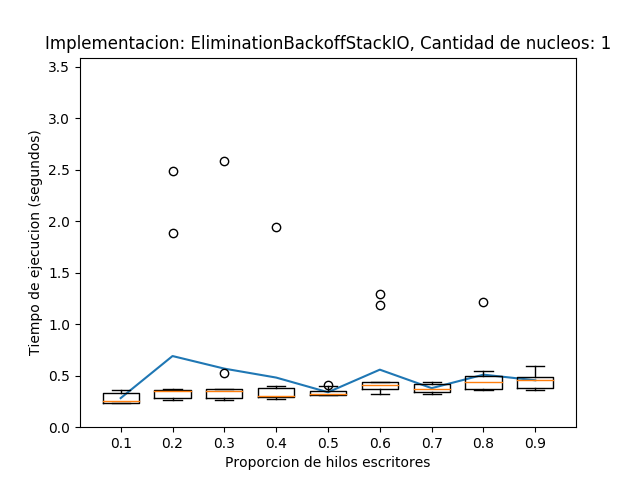
\includegraphics[width=\textwidth]{images/pushPercentages/plots/expEBSIO-1}
        \caption{Resultados para EBS sobre IO}
        \label{subfig:pushPercentages-ebsio-1}
    \end{subfigure}
    ~
    \begin{subfigure}[b]{0.49\textwidth}
        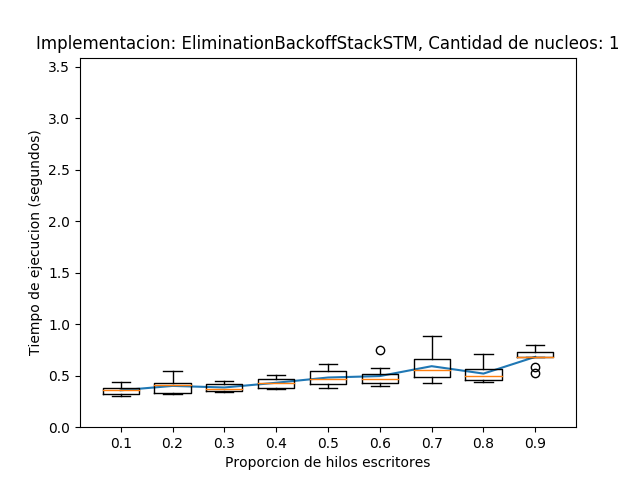
\includegraphics[width=\textwidth]{images/pushPercentages/plots/expEBSSTM-1}
        \caption{Resultados para EBS sobre STM}
        \label{subfig:pushPercentages-ebsstm-1}
    \end{subfigure}
    \begin{subfigure}[b]{0.49\textwidth}
        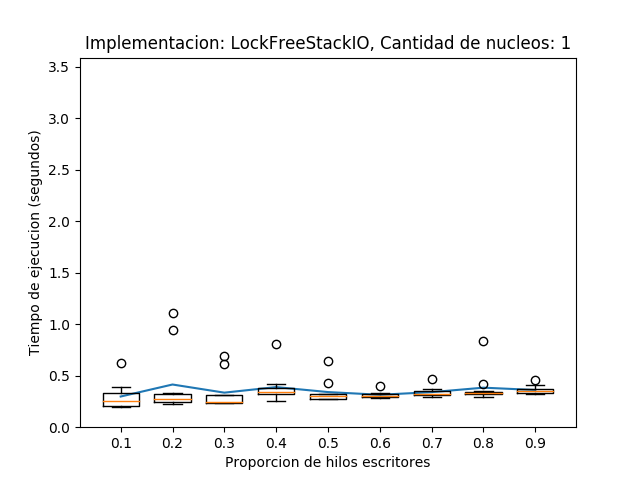
\includegraphics[width=\textwidth]{images/pushPercentages/plots/expLFSIO-1}
        \caption{Resultados para LFS sobre IO}
        \label{subfig:pushPercentages-lfsio-1}
    \end{subfigure}
    ~
    \begin{subfigure}[b]{0.49\textwidth}
        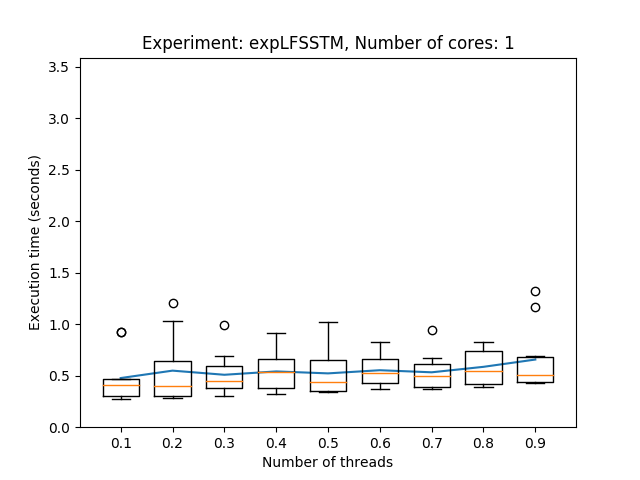
\includegraphics[width=\textwidth]{images/pushPercentages/plots/expLFSSTM-1}
        \caption{Resultados para LFS sobre STM}
        \label{subfig:pushPercentages-lfsstm-1}
    \end{subfigure}
    \begin{subfigure}[b]{0.49\textwidth}
        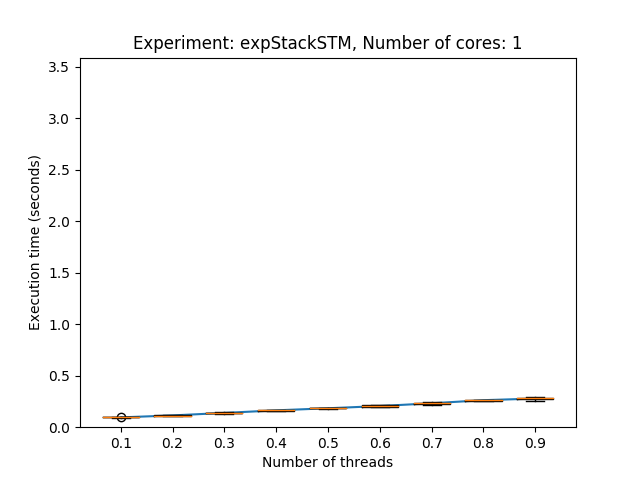
\includegraphics[width=\textwidth]{images/pushPercentages/plots/expStackSTM-1}
        \caption{Resultados para LFS sobre STM}
        \label{subfig:pushPercentages-stackstm-1}
    \end{subfigure}
    \caption{Comparación de implementaciones IO vs STM del experimento \mintinline{haskell}{pushPercentages} (1 núcleo de ejecución)}
    \label{fig:pushPercentages-boxplots-1}
\end{figure}

\begin{figure}[t]
    \centering
    \begin{subfigure}[b]{0.49\textwidth}
        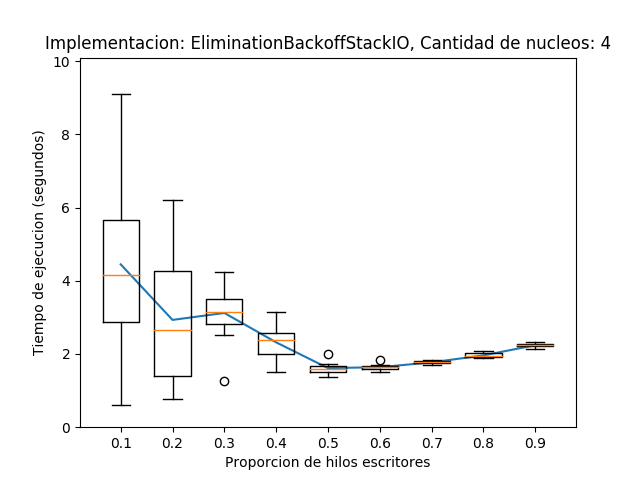
\includegraphics[width=\textwidth]{images/pushPercentages/plots/expEBSIO-4}
        \caption{Resultados para EBS sobre IO}
        \label{subfig:pushPercentages-ebsio-4}
    \end{subfigure}
    ~
    \begin{subfigure}[b]{0.49\textwidth}
        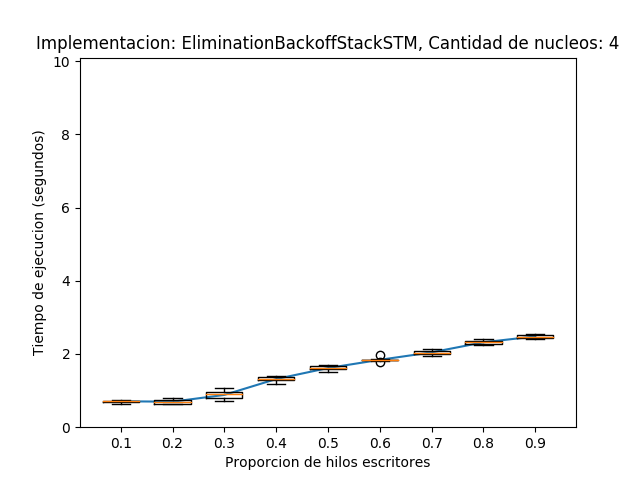
\includegraphics[width=\textwidth]{images/pushPercentages/plots/expEBSSTM-4}
        \caption{Resultados para EBS sobre STM}
        \label{subfig:pushPercentages-ebsstm-4}
    \end{subfigure}
    \begin{subfigure}[b]{0.49\textwidth}
        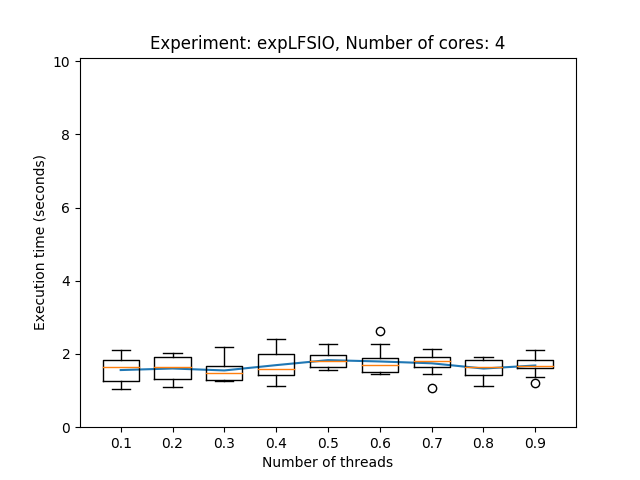
\includegraphics[width=\textwidth]{images/pushPercentages/plots/expLFSIO-4}
        \caption{Resultados para LFS sobre IO}
        \label{subfig:pushPercentages-lfsio-4}
    \end{subfigure}
    ~
    \begin{subfigure}[b]{0.49\textwidth}
        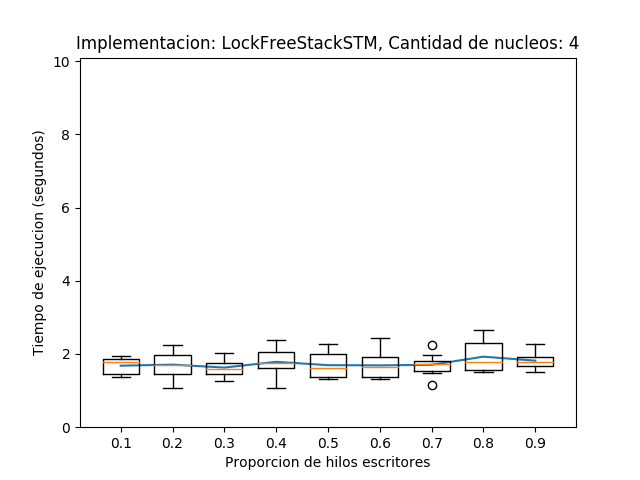
\includegraphics[width=\textwidth]{images/pushPercentages/plots/expLFSSTM-4}
        \caption{Resultados para LFS sobre STM}
        \label{subfig:pushPercentages-lfsstm-4}
    \end{subfigure}
    \begin{subfigure}[b]{0.49\textwidth}
        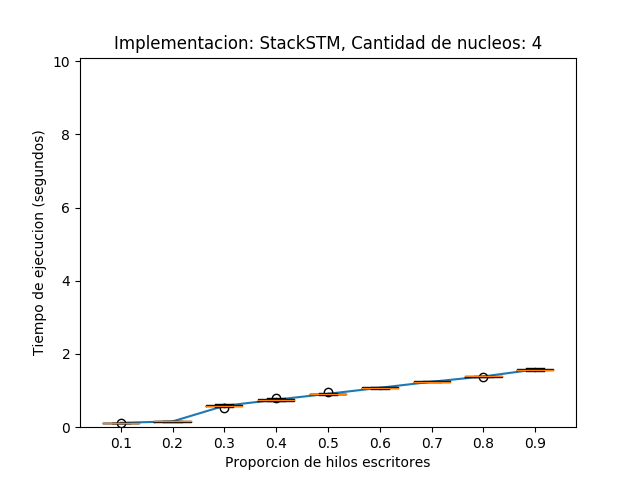
\includegraphics[width=\textwidth]{images/pushPercentages/plots/expStackSTM-4}
        \caption{Resultados para LFS sobre STM}
        \label{subfig:pushPercentages-stackstm-4}
    \end{subfigure}
    \caption{Comparación de implementaciones IO vs STM del experimento \mintinline{haskell}{pushPercentages} (4 núcleos de ejecución)}
    \label{fig:pushPercentages-boxplots-4}
\end{figure}

\section{Experimento \texttt{numberOfThreads}}

El experimento \texttt{numberOfThreads} estudia el comportamiento del tiempo de ejecución a medida que varía la cantidad total de hilos del experimento. En este experimento, la cantidad de operaciones totales aumenta a medida que aumentan los hilos ya que cada hilo que se agrega realiza una cantidad fija de operaciones. En las figuras \ref{fig:numberOfThreads-boxplots-1} y \ref{fig:numberOfThreads-boxplots-4} se presentan los resultados de cada implementación con diagramas \emph{boxplot} para las corridas realizadas en 1 y 4 núcleos respectivamente.

\begin{figure}[t]
    \centering
    \begin{subfigure}[b]{0.49\textwidth}
        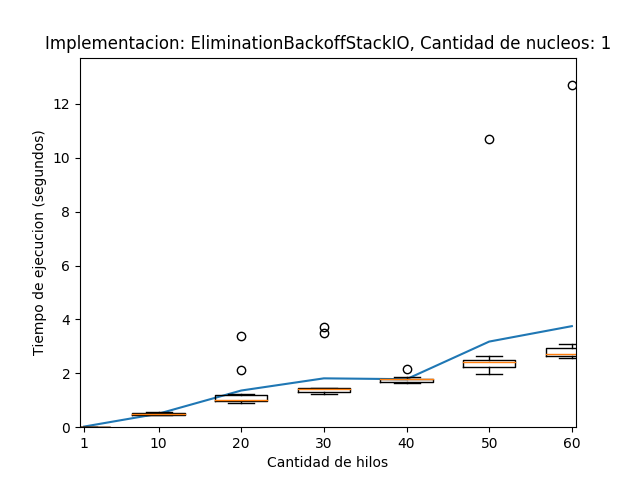
\includegraphics[width=\textwidth]{images/numberOfThreads/plots/expEBSIO-1}
        \caption{Resultados para EBS sobre IO}
        \label{subfig:numberOfThreads-ebsio-1}
    \end{subfigure}
    ~
    \begin{subfigure}[b]{0.49\textwidth}
        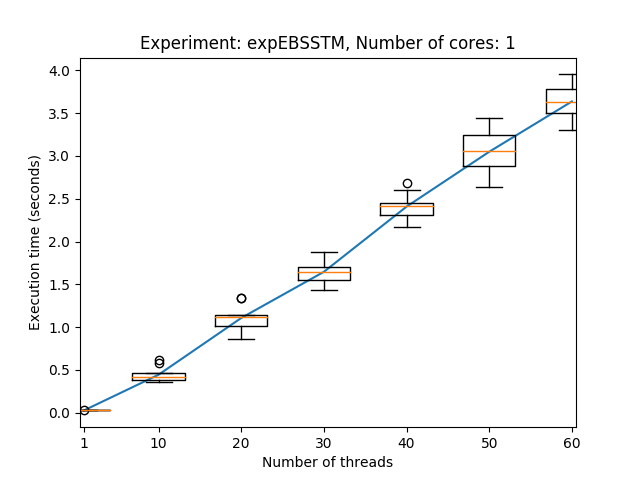
\includegraphics[width=\textwidth]{images/numberOfThreads/plots/expEBSSTM-1}
        \caption{Resultados para EBS sobre STM}
        \label{subfig:numberOfThreads-ebsstm-1}
    \end{subfigure}
    \begin{subfigure}[b]{0.49\textwidth}
        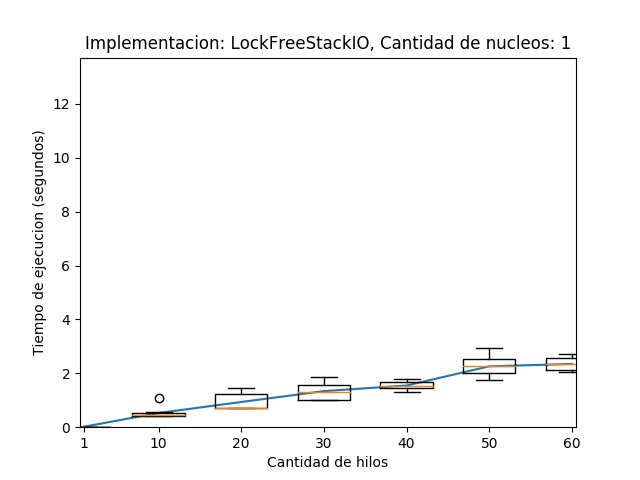
\includegraphics[width=\textwidth]{images/numberOfThreads/plots/expLFSIO-1}
        \caption{Resultados para LFS sobre IO}
        \label{subfig:numberOfThreads-lfsio-1}
    \end{subfigure}
    ~
    \begin{subfigure}[b]{0.49\textwidth}
        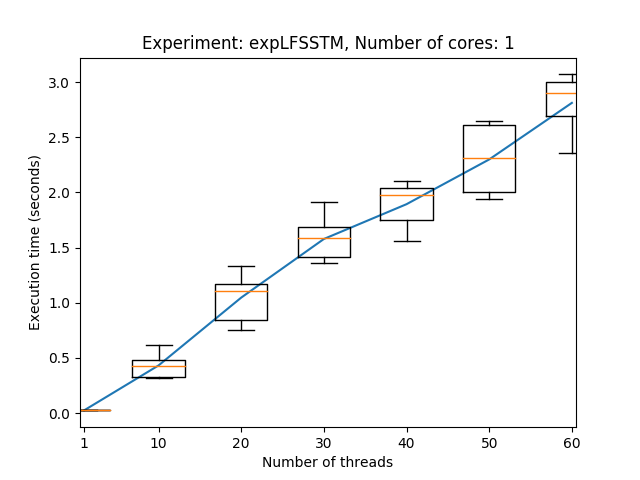
\includegraphics[width=\textwidth]{images/numberOfThreads/plots/expLFSSTM-1}
        \caption{Resultados para LFS sobre STM}
        \label{subfig:numberOfThreads-lfsstm-1}
    \end{subfigure}
    \begin{subfigure}[b]{0.49\textwidth}
        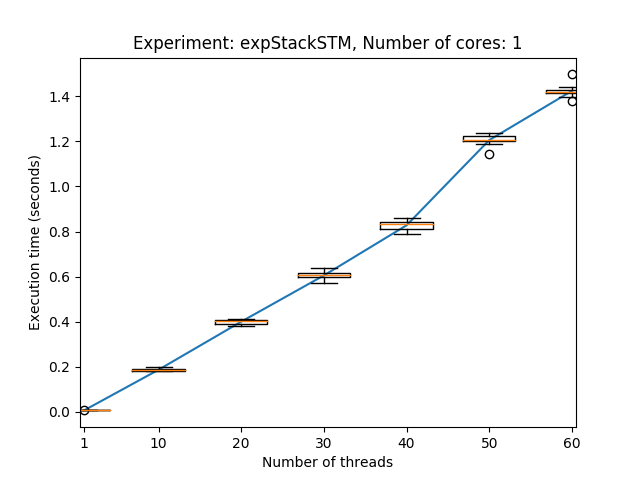
\includegraphics[width=\textwidth]{images/numberOfThreads/plots/expStackSTM-1}
        \caption{Resultados para LFS sobre STM}
        \label{subfig:numberOfThreads-stackstm-1}
    \end{subfigure}
    \caption{Comparación de implementaciones IO vs STM del experimento \mintinline{haskell}{numberOfThreads} (1 núcleo de ejecución)}
    \label{fig:numberOfThreads-boxplots-1}
\end{figure}

\begin{figure}[t]
    \centering
    \begin{subfigure}[b]{0.49\textwidth}
        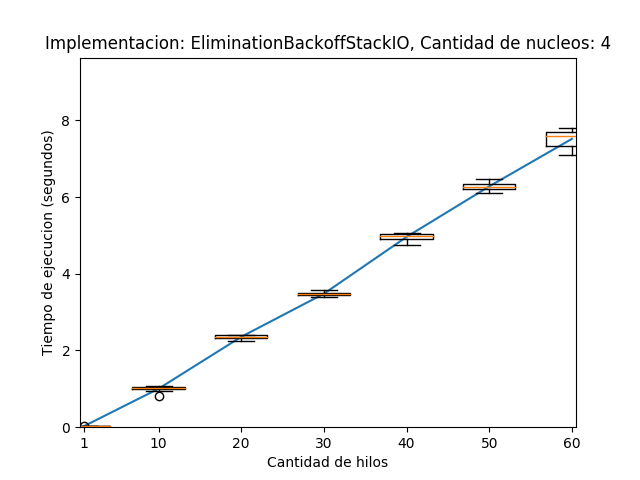
\includegraphics[width=\textwidth]{images/numberOfThreads/plots/expEBSIO-4}
        \caption{Resultados para EBS sobre IO}
        \label{subfig:numberOfThreads-ebsio-4}
    \end{subfigure}
    ~
    \begin{subfigure}[b]{0.49\textwidth}
        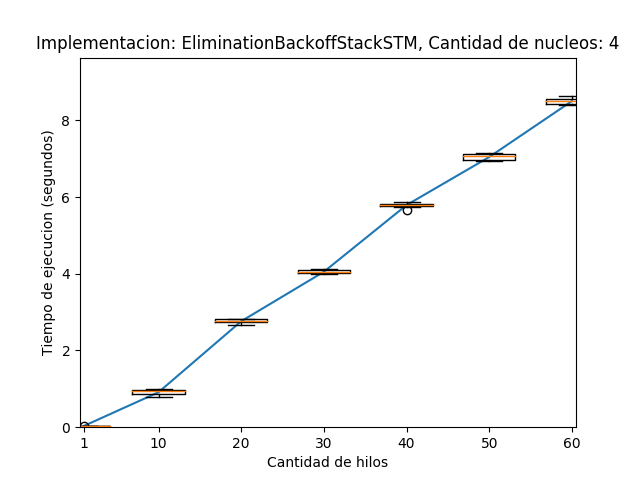
\includegraphics[width=\textwidth]{images/numberOfThreads/plots/expEBSSTM-4}
        \caption{Resultados para EBS sobre STM}
        \label{subfig:numberOfThreads-ebsstm-4}
    \end{subfigure}
    \begin{subfigure}[b]{0.49\textwidth}
        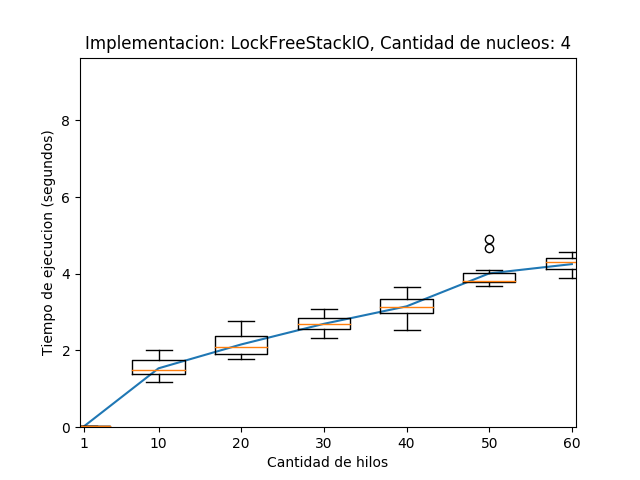
\includegraphics[width=\textwidth]{images/numberOfThreads/plots/expLFSIO-4}
        \caption{Resultados para LFS sobre IO}
        \label{subfig:numberOfThreads-lfsio-4}
    \end{subfigure}
    ~
    \begin{subfigure}[b]{0.49\textwidth}
        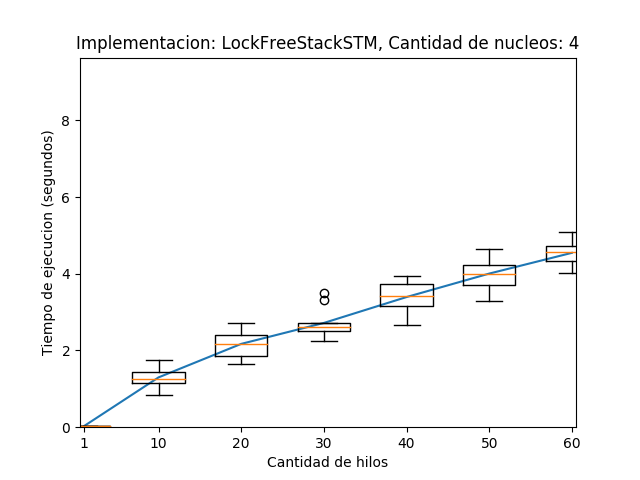
\includegraphics[width=\textwidth]{images/numberOfThreads/plots/expLFSSTM-4}
        \caption{Resultados para LFS sobre STM}
        \label{subfig:numberOfThreads-lfsstm-4}
    \end{subfigure}
    \begin{subfigure}[b]{0.49\textwidth}
        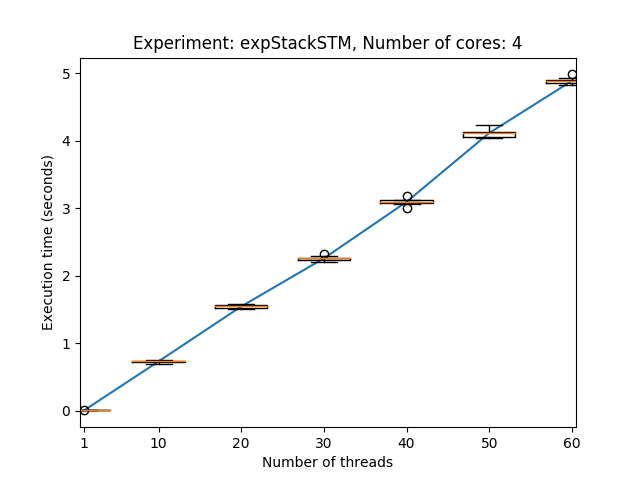
\includegraphics[width=\textwidth]{images/numberOfThreads/plots/expStackSTM-4}
        \caption{Resultados para LFS sobre STM}
        \label{subfig:numberOfThreads-stackstm-4}
    \end{subfigure}
    \caption{Comparación de implementaciones IO vs STM del experimento \mintinline{haskell}{numberOfThreads} (4 núcleos de ejecución)}
    \label{fig:numberOfThreads-boxplots-4}
\end{figure}


\section{Experimento \texttt{numberOfThreadsDist}}
El experimento \texttt{numberOfThreadsDist} estudia el comportamiento del tiempo de ejecución a medida que varía la cantidad total de hilos del experimento. En este experimento, la cantidad de operaciones totales se mantiene constante y se distribuye entre los hilos de ejecución. En las figuras \ref{fig:numberOfThreadsDist-boxplots-1} y \ref{fig:numberOfThreadsDist-boxplots-4} se presentan los resultados de cada implementación con diagramas \emph{boxplot} para las corridas realizadas en 1 y 4 núcleos respectivamente.


\begin{figure}[t]
    \centering
    \begin{subfigure}[b]{0.49\textwidth}
        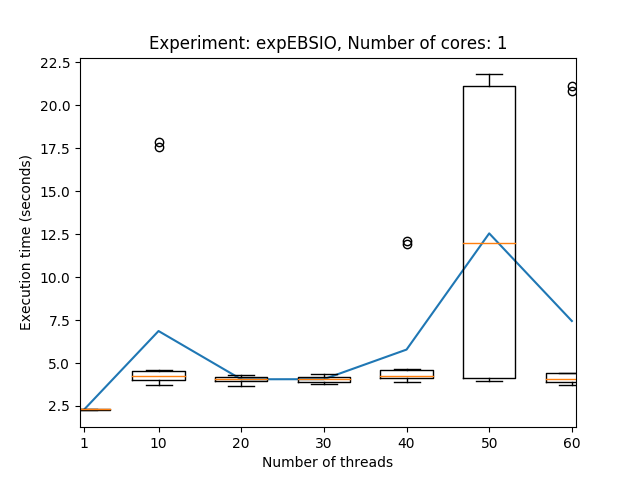
\includegraphics[width=\textwidth]{images/numberOfThreadsDist/plots/expEBSIO-1}
        \caption{Resultados para EBS sobre IO}
        \label{subfig:numberOfThreadsDist-ebsio-1}
    \end{subfigure}
    ~
    \begin{subfigure}[b]{0.49\textwidth}
        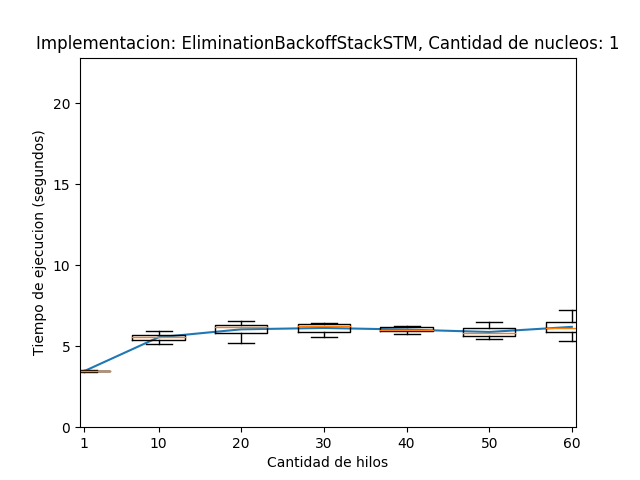
\includegraphics[width=\textwidth]{images/numberOfThreadsDist/plots/expEBSSTM-1}
        \caption{Resultados para EBS sobre STM}
        \label{subfig:numberOfThreadsDist-ebsstm-1}
    \end{subfigure}
    \begin{subfigure}[b]{0.49\textwidth}
        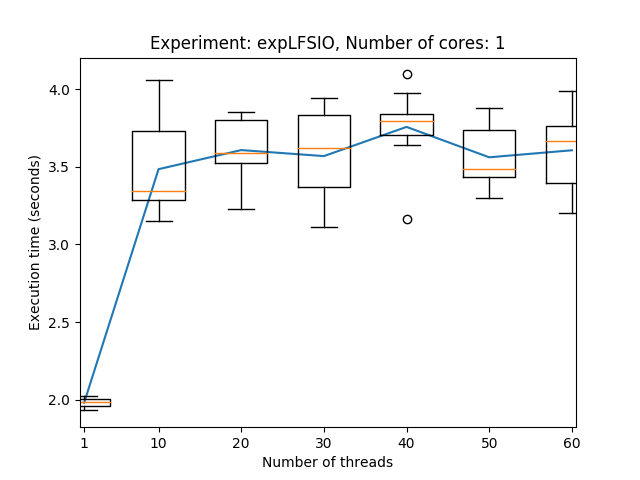
\includegraphics[width=\textwidth]{images/numberOfThreadsDist/plots/expLFSIO-1}
        \caption{Resultados para LFS sobre IO}
        \label{subfig:numberOfThreadsDist-lfsio-1}
    \end{subfigure}
    ~
    \begin{subfigure}[b]{0.49\textwidth}
        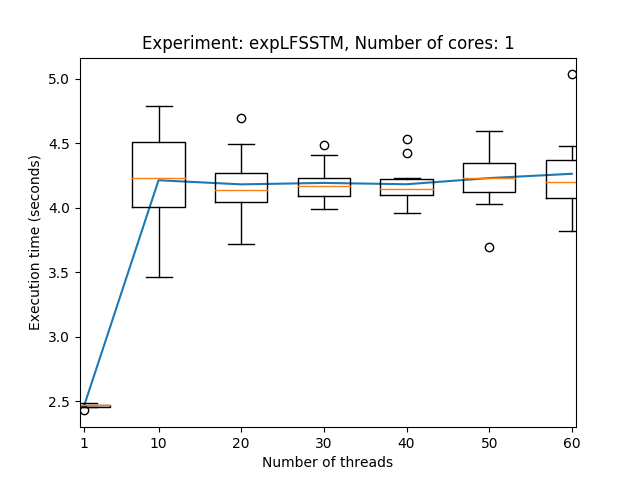
\includegraphics[width=\textwidth]{images/numberOfThreadsDist/plots/expLFSSTM-1}
        \caption{Resultados para LFS sobre STM}
        \label{subfig:numberOfThreadsDist-lfsstm-1}
    \end{subfigure}
    \begin{subfigure}[b]{0.49\textwidth}
        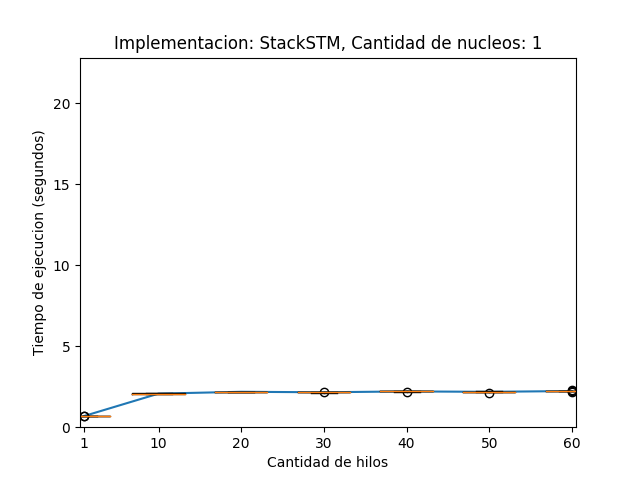
\includegraphics[width=\textwidth]{images/numberOfThreadsDist/plots/expStackSTM-1}
        \caption{Resultados para LFS sobre STM}
        \label{subfig:numberOfThreadsDist-stackstm-1}
    \end{subfigure}
    \caption{Comparación de implementaciones IO vs STM del experimento \mintinline{haskell}{numberOfThreadsDist} (1 núcleo de ejecución)}
    \label{fig:numberOfThreadsDist-boxplots-1}
\end{figure}

\begin{figure}[t]
    \centering
    \begin{subfigure}[b]{0.49\textwidth}
        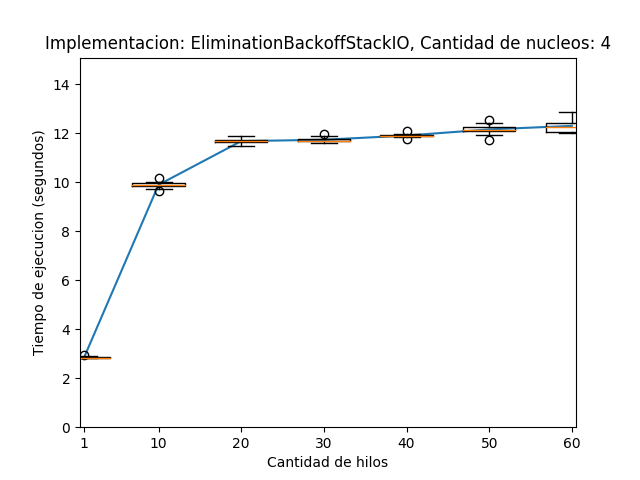
\includegraphics[width=\textwidth]{images/numberOfThreadsDist/plots/expEBSIO-4}
        \caption{Resultados para EBS sobre IO}
        \label{subfig:numberOfThreadsDist-ebsio-4}
    \end{subfigure}
    ~
    \begin{subfigure}[b]{0.49\textwidth}
        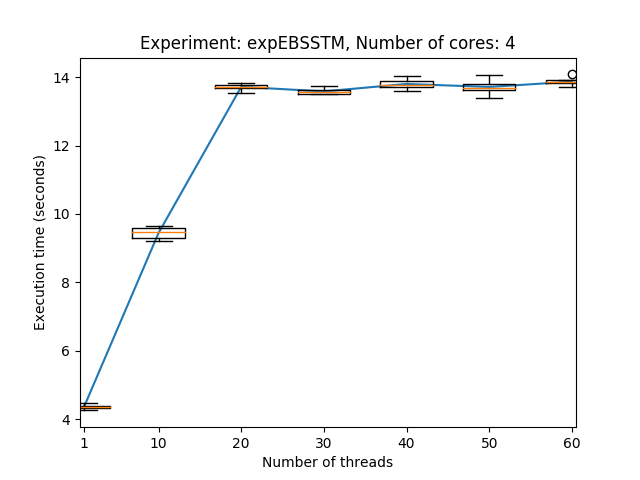
\includegraphics[width=\textwidth]{images/numberOfThreadsDist/plots/expEBSSTM-4}
        \caption{Resultados para EBS sobre STM}
        \label{subfig:numberOfThreadsDist-ebsstm-4}
    \end{subfigure}
    \begin{subfigure}[b]{0.49\textwidth}
        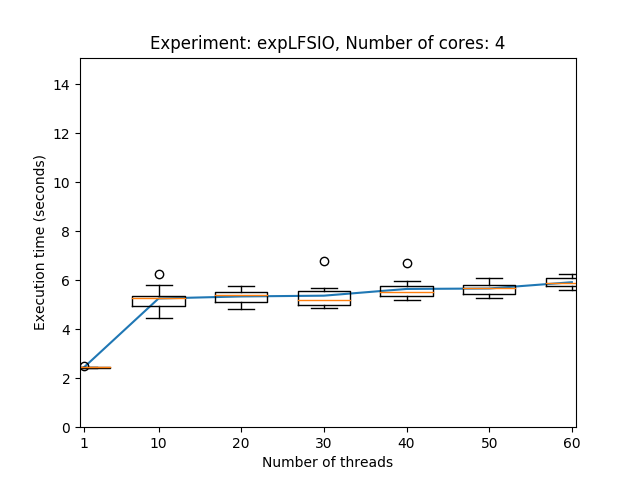
\includegraphics[width=\textwidth]{images/numberOfThreadsDist/plots/expLFSIO-4}
        \caption{Resultados para LFS sobre IO}
        \label{subfig:numberOfThreadsDist-lfsio-4}
    \end{subfigure}
    ~
    \begin{subfigure}[b]{0.49\textwidth}
        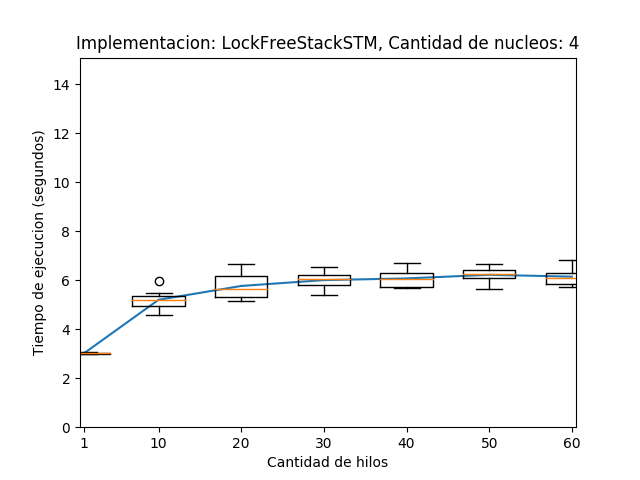
\includegraphics[width=\textwidth]{images/numberOfThreadsDist/plots/expLFSSTM-4}
        \caption{Resultados para LFS sobre STM}
        \label{subfig:numberOfThreadsDist-lfsstm-4}
    \end{subfigure}
    \begin{subfigure}[b]{0.49\textwidth}
        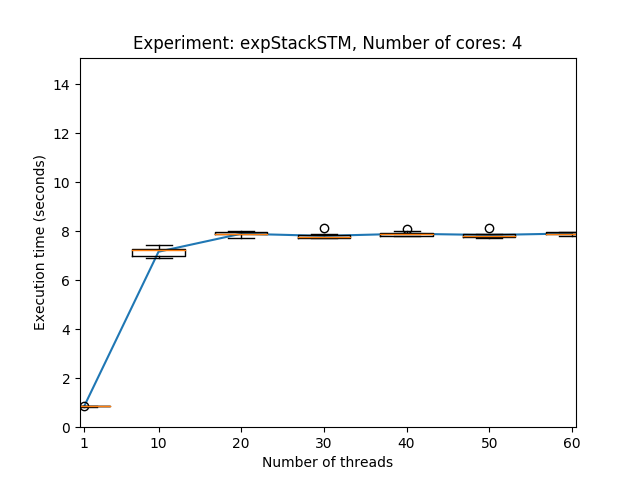
\includegraphics[width=\textwidth]{images/numberOfThreadsDist/plots/expStackSTM-4}
        \caption{Resultados para LFS sobre STM}
        \label{subfig:numberOfThreadsDist-stackstm-4}
    \end{subfigure}
    \caption{Comparación de implementaciones IO vs STM del experimento \mintinline{haskell}{numberOfThreadsDist} (4 núcleos de ejecución)}
    \label{fig:numberOfThreadsDist-boxplots-4}
\end{figure}

\end{appendices}